\documentclass[12pt, titlepage, oneside]{article}
\usepackage[letterpaper, margin=1in]{geometry}
\usepackage{siunitx, booktabs, amsmath, enumitem, pdfpages, tabularx,caption, graphicx, pgfplots, textcomp}
\usepackage[siunitx]{circuitikz}
\sisetup{detect-weight=true, detect-family=true}
\usepackage{wrapfig}
\usepackage{mathrsfs}
\setlength\parindent{0pt}
\let\oldhat\hat
\let\oldvec\vec
\newcommand{\cross}{\bm{\times}}
\renewcommand{\hat}[1]{\oldhat{\mathbf{#1}}}
\usepackage{bm}
\renewcommand{\vec}[1]{\oldvec{\bm{#1}}}
\renewcommand{\hat}[1]{\oldhat{\bm{#1}}}
\renewcommand{\b}[1]{\textbf{#1}}

\begin{document}
	\section*{30.1 The Biot-Savart Law}

	The mathematical expression for the magnetic field for some point in space can be shown in terms of the current that produces that field. The expression is based of experimental observations for the magnetic field, $d\vec{B}$ at some point $P$ with a length of wire d$\vec{s}$ carrying a steady current $I$.\\
	
	It was found that,
	
	\begin{wrapfigure}[0]{r}{0.4\textwidth}
		\begin{center}
			\vspace{-4cm}
			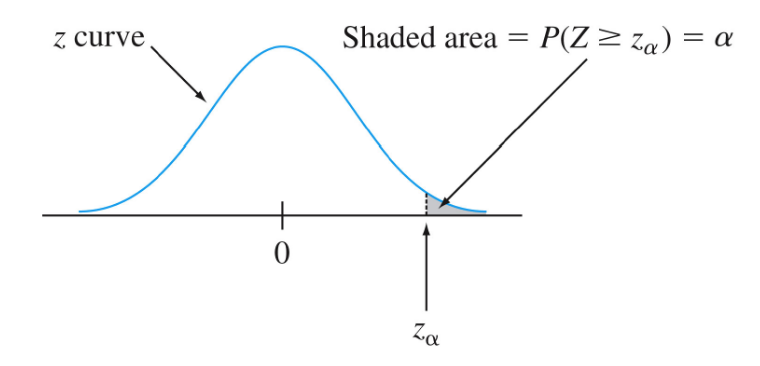
\includegraphics[scale=.4]{1.png}
				\end{center}
	\end{wrapfigure}
	\begin{itemize}
	\item The vector $d\vec{B}$ is perpendicular to both $d\vec{s}$ (which points in the firection of the current) and to the unit vector $\hat{r}$ which is directed from $d\vec{r} $ to $P$.
	\item The magnitude of  $d\vec{B}$ is inversely proportional to $r^2$, where $r$ is the distance from $d\vec{s}$ to $P$.
	\item The magnitude of $d\vec{B}$ is proportional to the current $I$ and to the magnitude $ds$ of the length element $d\vec{s}$.
	\item The magnitude of $d\vec{B}$ is proportional to $\sin \theta$, where $\theta $ is the angle between the vectors $d\vec{s}$ and $\hat{r}$. From these observations the scientists were able to find a mathematical expression, 
\end{itemize}


			\noindent\fbox{%
		\parbox{\textwidth}{%
			\textbf{Biot-Savart Law}
	\begin{align}
	d\vec{B} = \frac{\mu_0}{4\pi} \cdot \frac{I d\vec{s} \times \hat{r}}{r^2}
	\end{align}
	where $\mu_0$ is the \textbf{permeability of free space}:
	\begin{align}
	\mu_0 = 4\pi \times 10^{-7} \si{T m\per A}
	\end{align}
	A more general form of the law would be,
	\begin{align}
	\vec{B} = \frac{I\mu_0}{4\pi} \cdot \int \frac{d\vec{s} \times \hat{r}}{r^2}
	\end{align}
}}\\


The methods for solving biot-Savart law are the following,
\begin{itemize}
\item Infinite Rod or Wire
\item Centre of a Magnetic Ring of $\theta$ degrees
\item Magnetic Ring placed along the $zy$ plane at a horizontal distance $x$ 
\end{itemize}
The field direction must be evaluated by hand using the right hand rule, and they can be added up vectorially to provide a net field at a certain point.
\newpage 


\begin{wrapfigure}{r}{0.3\textwidth}
	\begin{center}
		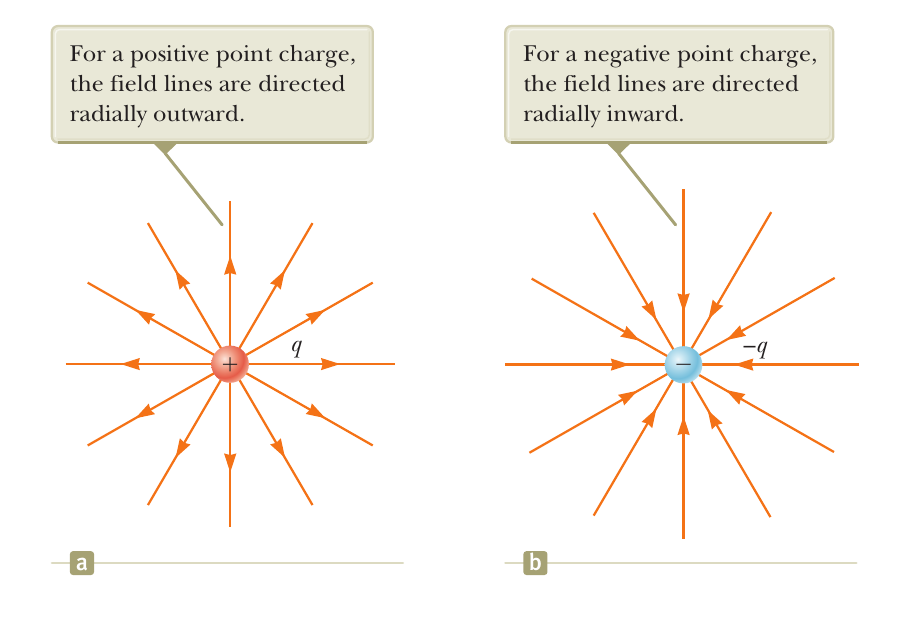
\includegraphics[scale=.4]{2.png}
	\end{center}
\end{wrapfigure}
The Biots-Savart's  equation for an \b{infinite rod}, we evaluate the field at $P$
\begin{align*}
| d\vec{s}  \cross \hat{r} |\hat{k} = \Bigg[dx \sin\bigg(\frac{\pi}{2}-\theta\bigg)\Bigg] \hat{k} = (dx \cos(\theta))\hat{k}
\end{align*}
Substitute into the general equation,
\begin{equation}
d\vec{B} = (dB)\hat{k} = \frac{\mu_0 I}{4\pi} \cdot \frac{dx \cos\theta}{r^2} \hat{k}
\end{equation}
Using trigonometry we find two relationships,
\begin{equation}
r = \frac{a}{\cos\theta} \hspace{2cm}
x = -a \tan \theta
\end{equation}
Find the differential $dx$
\begin{equation}
dx = -a \sec^2\theta \, d\theta = \frac{-a\, d\theta}{\cos^2\theta}
\end{equation}
Replacing our current expression for $dx$ in equation 4,
\begin{equation}
dB = -\frac{\mu_0 I }{4\pi} \left(\frac{a \, d\theta }{\cos^2\theta}\right) \left(\frac{\cos^2\theta}{a^2} \right) \cos\theta = -\frac{\mu_0 I}{4\pi a} \cos\theta \, d\theta
\end{equation}
We can integrate over the two angles, we can assume that the angles would be $\pi/2$ and $-\pi/2$. Therefore, this is essentially finding the field about an infinitely long wire. We get our final answer as,
\begin{equation}
B = \frac{\mu_0 I}{2\pi a}
\end{equation}
Where a is the \textbf{distance} from the wire to a point $P$
\\


\begin{wrapfigure}{r}{0.3\textwidth}
	\begin{center}\vspace{-1cm}
		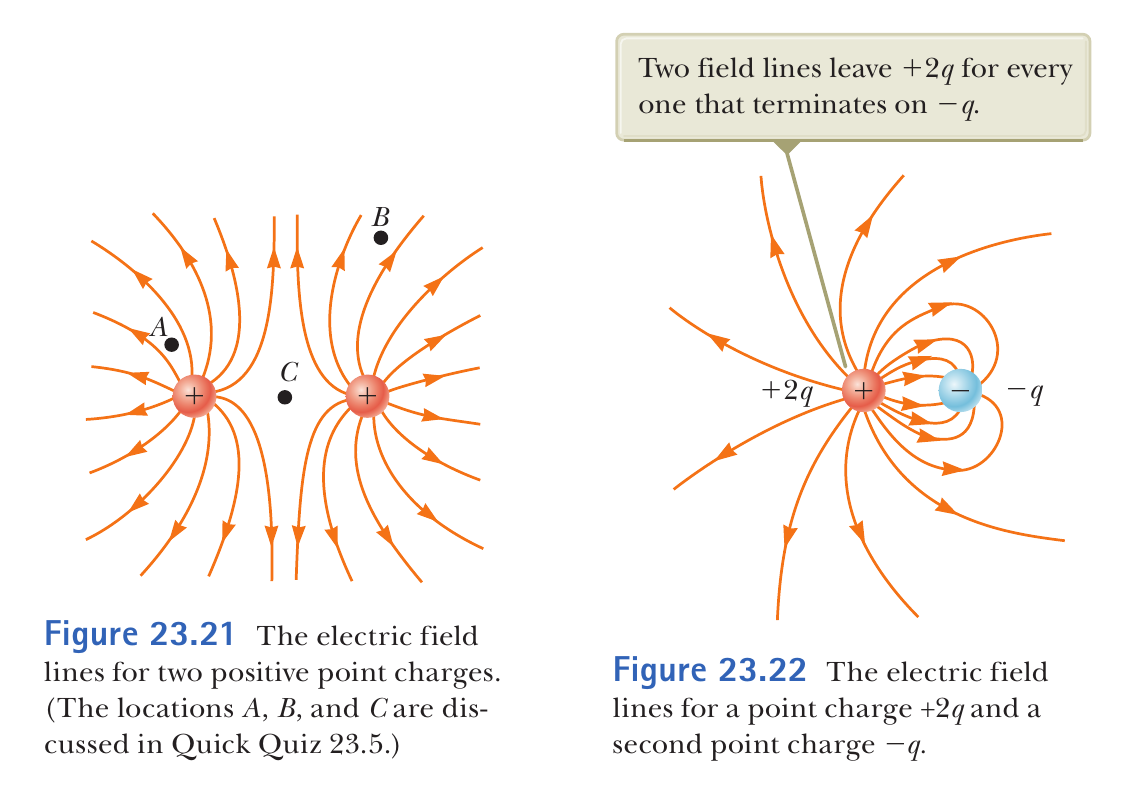
\includegraphics[scale=.5]{3.png}
	\end{center}
\end{wrapfigure}
The biot-Savart's equation for a \b{curved wire segment}, we notice that each element $d\vec{s}$ is the same distance, $a$, from point $O$. Since every $d\vec{s}$ is perpendicular to $\hat{r}$,
\begin{equation}
|d\vec{s}\cross \hat{r}| = ds
\end{equation}
Plugging into the general equation, 
\begin{equation}
dB = \frac{\mu_0}{4\pi}\cdot\frac{I \, ds}{a^2}
\end{equation}
Solving for B, remembering $s = a\theta$
\begin{align}
B = \frac{\mu_0 I}{4\pi a^2}\int ds = \frac{\mu_0 I}{4\pi a^2}\, s = \frac{\mu_0 I}{4\pi a}\,\theta
\end{align}

\newpage
The biot-Savart's equation for a \b{magnetic field on the axis of a circuilar current loop}.
\begin{center}
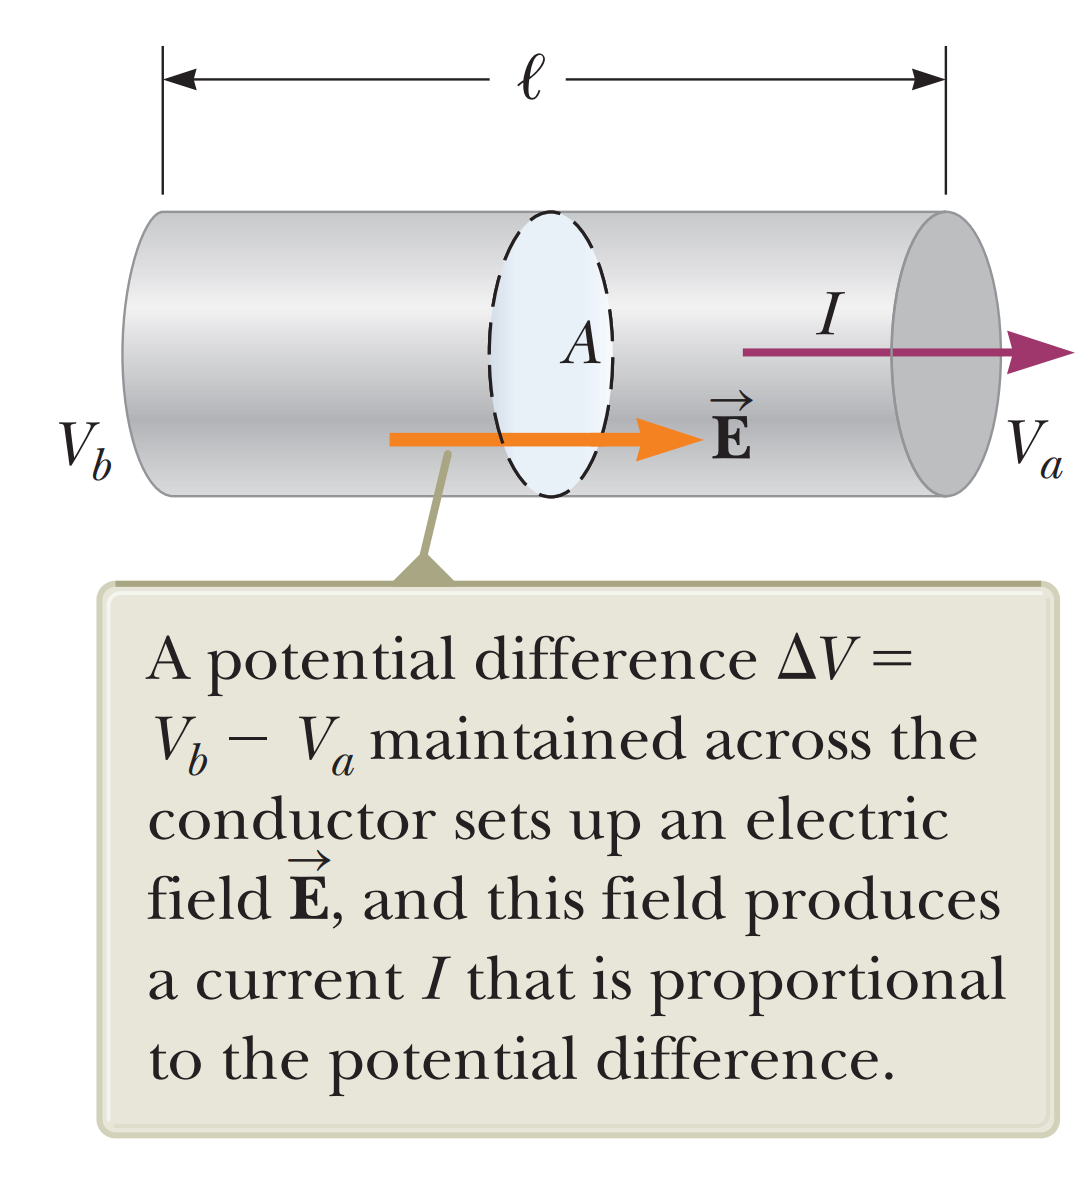
\includegraphics[scale=0.4]{4.png}
\end{center}

Consider a circular wire loop of radius $a$ located in the $yz$ plane and carrying a steady current $I$. To find the fource at $P$ which is a distance $x$ away, we see that,

\begin{equation}
|d\vec{s} \cross \hat{r}| = ds
\end{equation}

The distance from $P$ to al points on the loop is,

\begin{equation}
s^2 = a^2 + x^2
\end{equation}

Plugging into the general formula,

\begin{equation}
dB = \frac{\mu_0 I}{r^2} \frac{|d\vec{s}\cross\hat{r}|}{r^2} = \frac{\mu_0 I}{r^2} \frac{ds}{(a^2+x^2)}
\end{equation}
Take only the $B_x$ elememts as the $y$ elements cancel. Therefore, we can notice that,
\begin{equation}
dB_x =  \frac{\mu_0 I}{4\pi} \frac{ds}{(a^2+x^2)} \,\cos\theta
\end{equation}
Using trigonometry, we can notice that,
\begin{equation}
\cos\theta = \frac{a}{(x^2+a^2)^{1/2}}
\end{equation} 
Pluging this back in, we notice we would be required to integrate over every $d\vec{s}$ element, which is simply a integrating over a closed loop,
\begin{equation}
B_x = \frac{\mu_0 I}{4\pi} \oint \frac{ds}{a^2 + x^2} \left[ \frac{a}{(a^2+x^2)^{1/2}} \right] = \frac{\mu_0 I}{4\pi} \frac{a}{(a^2+x^2)^{3/2}} \oint ds	
\end{equation}
Notice that the total displacement $s = 2\pi a$,
\begin{equation}
B_x = \frac{\mu_0 I}{4\pi} \frac{a}{(a^2+x^2)^{3/2}}(4\pi a) = \frac{\mu_0 I a^2}{2(a^2+x^2)^{3/2}}
\end{equation}
Notice that if $x = 0$ such that the point $P$ is in the center of the magnetic ring,
\begin{equation}
B_x = \frac{\mu_0 I a^2}{2a^3} = \frac{\mu_0 I}{2a}
\end{equation}
Notice this was the same equation as the curved wire segment, if $\theta = 2\pi$ 


\section*{30.2 The Magnetic Force Between Two Parallel Conductors}  
The Force between two parallel conductors with the \b{same direction of current} would have an \b{attractive} force between them. Two parallel conductors with \b{different directions of current} would have \b{repelling force between them}. We can compute the magnitude of the force,

\begin{center}
	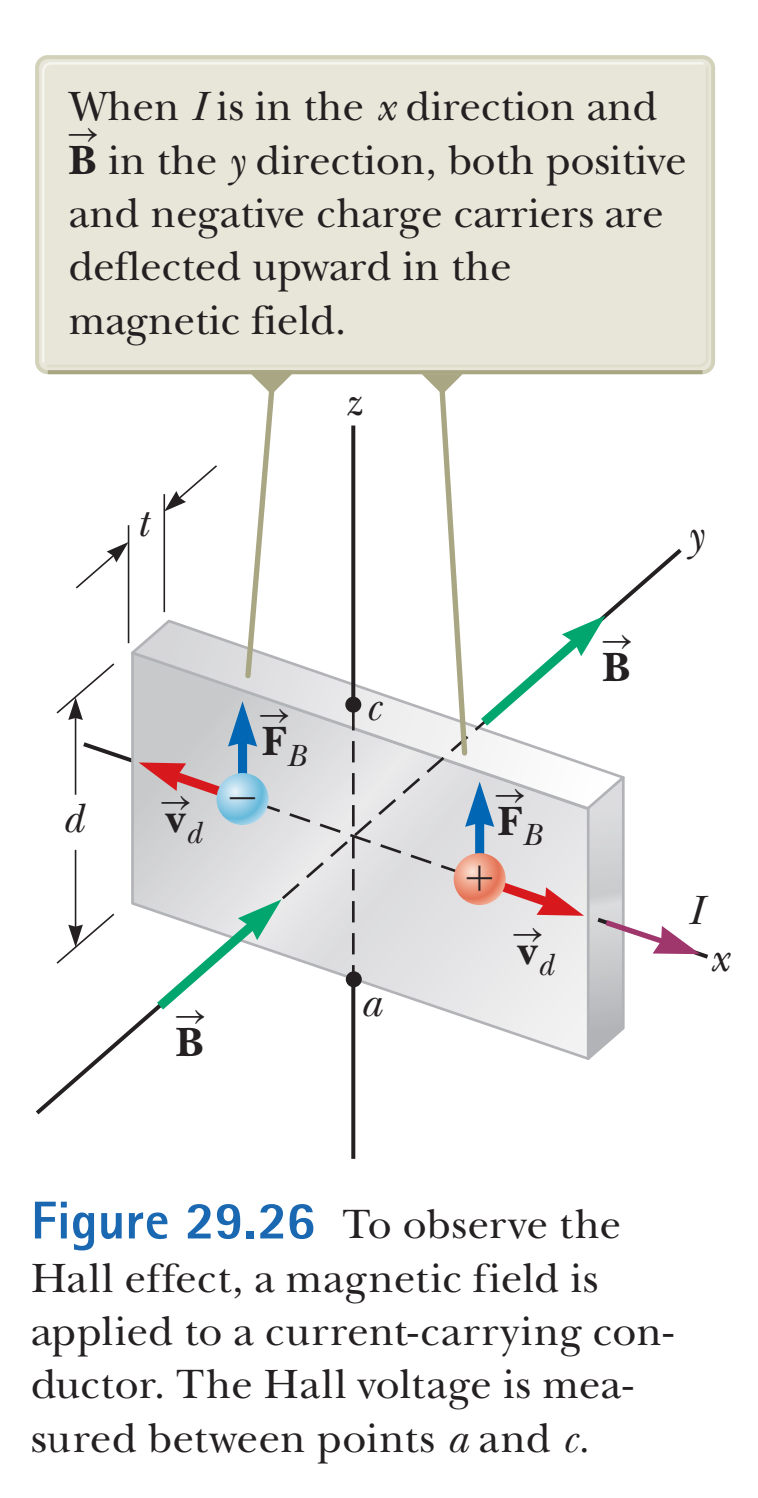
\includegraphics[scale=0.4]{5.png}
\end{center}
\begin{equation}
F_1 = I_1 l B_2 = I_1 l \left( \frac{\mu_0 I_2}{2\pi a} \right) = \frac{\mu_0 I_1 I_2}{2\pi a} l
\end{equation}

Sometimes there exists an infinite length we can use force per length,

\begin{equation}
\frac{F_B}{l} = \frac{\mu_0 I_1 I_2}{2\pi a}.
\end{equation}

The force between two parallel wires carrying a currents are separated by 1m is $\SI{2e-7}{N/m}$, the current in each wire is defined to be 1A 


The SI unit of charge, the \b{coulomb} is defined in terms of the ampere. When a conductor carries a steady current of 1 A, the quantity of charge that flows through a cross section of of the conductor in 1s is 1C.

\end{document}